% future/cpu.tex
% SPDX-License-Identifier: CC-BY-SA-3.0

\section{The Future of CPU Technology Ain't What it Used to Be}
\label{sec:future:The Future of CPU Technology Ain't What it Used to Be}

과거란 많은 기간의 경험을 거친 렌즈를 통해 보기에는 항상 매우 간단하고 순수해
보입니다.
그리고 2000년대 초는 Moore's Law 가 그땐 전통적이었던 CPU 클락 주파수의 증가를
가져오던 현상이 깨지기 시작하는 시점에 임박했던, 순수했던 시대였습니다.
아, 그때도 기술의 한계에 대한 가끔의 경고는 있었습니다만 그런 경고들은 수십년째
이어져 오고 있었습니다.
그걸 마음에 둔 채로, 다음의 시나리오들을 고려해 봅시다:
\iffalse

Years past always seem so simple and innocent when viewed through the
lens of many years of experience.
And the early 2000s were for the most part innocent of the impending
failure of Moore's Law to continue delivering the then-traditional
increases in CPU clock frequency.
Oh, there were the occasional warnings about the limits of technology,
but such warnings had been sounded for decades.
With that in mind, consider the following scenarios:
\fi

\begin{figure}[tb]
\centering
\resizebox{3in}{!}{
\includegraphics{cartoons/r-2014-CPU-future-uniprocessor-uber-alles}}
\caption{Uniprocessor \"Uber Alles}
\ContributedBy{Figure}{fig:future:Uniprocessor Uber Alles}{Melissa Broussard}
\end{figure}

\begin{figure}[tb]
\centering
\resizebox{3in}{!}{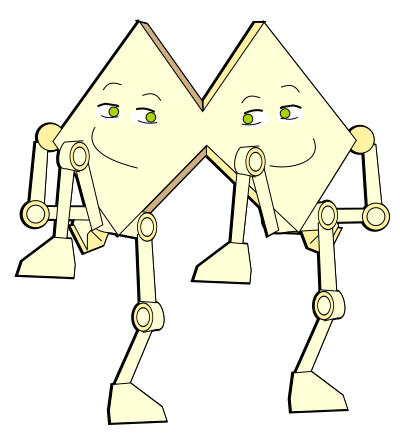
\includegraphics{cartoons/r-2014-CPU-Future-Multithreaded-Mania}}
\caption{Multithreaded Mania}
\ContributedBy{Figure}{fig:future:Multithreaded Mania}{Melissa Broussard}
\end{figure}

\begin{figure}[tb]
\centering
\resizebox{3in}{!}{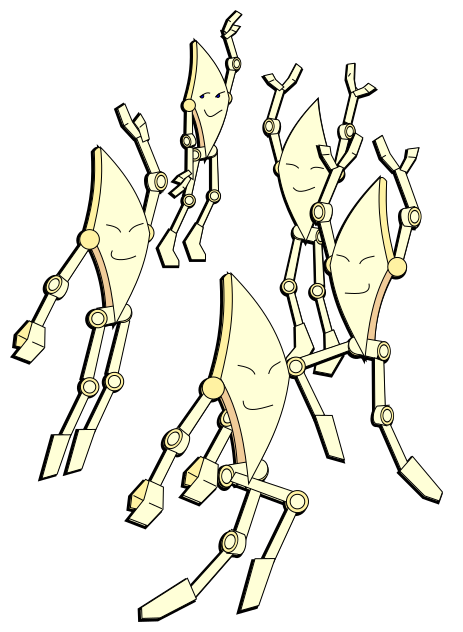
\includegraphics{cartoons/r-2014-CPU-Future-More-of-the-Same}}
\caption{More of the Same}
\ContributedBy{Figure}{fig:future:More of the Same}{Melissa Broussard}
\end{figure}

\begin{figure}[tb]
\centering
\resizebox{3in}{!}{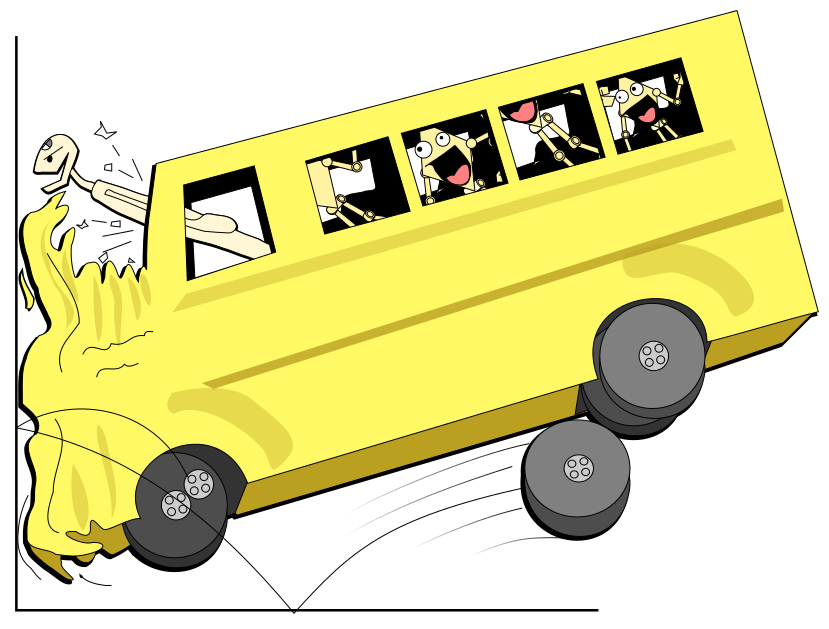
\includegraphics{cartoons/r-2014-CPU-Future-Crash-dummies}}
\caption{Crash Dummies Slamming into the Memory Wall}
\ContributedBy{Figure}{fig:future:Crash Dummies Slamming into the Memory Wall}{Melissa Broussard}
\end{figure}

\begin{enumerate}
\item	유니프로세서 \"Uber Alles
	(Figure~\ref{fig:future:Uniprocessor Uber Alles}),
\item	멀티쓰레드 매니아
	(Figure~\ref{fig:future:Multithreaded Mania}),
\item	더 많은 같은것들
	(Figure~\ref{fig:future:More of the Same}), 그리고
\item	메모리 장벽에 부닺치는 것들
	(Figure~\ref{fig:future:Crash Dummies Slamming into the Memory Wall}).
\iffalse

\item	Uniprocessor \"Uber Alles
	(Figure~\ref{fig:future:Uniprocessor Uber Alles}),
\item	Multithreaded Mania
	(Figure~\ref{fig:future:Multithreaded Mania}),
\item	More of the Same
	(Figure~\ref{fig:future:More of the Same}), and
\item	Crash Dummies Slamming into the Memory Wall
	(Figure~\ref{fig:future:Crash Dummies Slamming into the Memory Wall}).
\fi
\end{enumerate}

다음의 섹션들은 이 시나리오들 각각을 다룹니다.
\iffalse

Each of these scenarios are covered in the following sections.
\fi

\subsection{Uniprocessor \"Uber Alles}
\label{sec:future:Uniprocessor Uber Alles}

2004년에 이야기한 것~\cite{PaulEdwardMcKenneyPhD} 처럼:
\iffalse

As was said in 2004~\cite{PaulEdwardMcKenneyPhD}:
\fi

\begin{quote}
	이 시나리오에서, Moore's-Law 를 통한 CPU 클락 속도의 증가와 수평적으로
	확장되는 컴퓨팅의 계속된 발전의 조합은 SMP 시스템들을 무의미하게
	만듭니다.
	따라서 이 시나리오는 ``Uniprocessor \"Uber Alles'', 말 그대로 다른
	모든것보다 나은 유니프로세서라고 불립니다.

	이런 유니프로세서 시스템들은 인스트럭션 오버헤드만이 문제가 될텐데,
	메모리 배리어, cache thrashing, 그리고 cache contention 은 단일 CPU
	시스템에서는 문제가 없기 때문입니다.
	이 시나리오 상에서, RCU 는 NMI 들과의 상호작용과 같은 간단한 부분에서만
	유용할 것입니다.
	이미 RCU 를 구현한 운영체제는 그대로 RCU 를 가지고 있어도 되겠지만, RCU
	가 존재하지 않는 운영 체제가 RCU 를 적용해야 할지는 분명치 않습니다.

	하지만, 최근의 멀티쓰레드 사용 CPU 의 발전은 이 시나리오가 이뤄질
	가능성은 적다고 이야기 합니다.
	\iffalse

	In this scenario, the combination of Moore's-Law increases in CPU
	clock rate and continued progress in horizontally scaled computing
	render SMP systems irrelevant.
	This scenario is therefore dubbed ``Uniprocessor \"Uber
	Alles'', literally, uniprocessors above all else.

	These uniprocessor systems would be subject only to instruction
	overhead, since memory barriers, cache thrashing, and contention
	do not affect single-CPU systems.
	In this scenario, RCU is useful only for niche applications, such
	as interacting with NMIs.
	It is not clear that an operating system lacking RCU would see
	the need to adopt it, although operating
	systems that already implement RCU might continue to do so.

	However, recent progress with multithreaded CPUs seems to indicate
	that this scenario is quite unlikely.
	\fi
\end{quote}

실제로 그렇게 되진 않을 겁니다!
하지만 더 커다란 소프트웨어 커뮤니티는 그들이 병렬성을 포용해야 한다는 사실을
받아들이기를 꺼려했는데, 이는 이 커뮤니티가 Moore's-Law 로 인한 CPU 코어 클락
주파수 상승의 ``공짜 점심'' 이 정말로 끝났다는 결론을 내리기 전이었습니다.
잊지 마세요: 믿음은 감정이지, 이성적이고 기술적인 생각 과정의 결과가 아닐 수
있습니다!
\iffalse

Unlikely indeed!
But the larger software community was reluctant to accept the fact that
they would need to embrace parallelism, and so it was some time before
this community concluded that the ``free lunch'' of Moore's-Law-induced
CPU core-clock frequency increases was well and truly finished.
Never forget: belief is an emotion, not necessarily the result of a
rational technical thought process!
\fi

\subsection{Multithreaded Mania}
\label{sec:future:Multithreaded Mania}

역시 2004년의 이야기~\cite{PaulEdwardMcKenneyPhD} 에서:
\iffalse

Also from 2004~\cite{PaulEdwardMcKenneyPhD}:
\fi

\begin{quote}
	Uniprocessor \"Uber Alles 의 덜 극단적인 변종은 하드웨어 멀티쓰레딩을
	제공하는 유니프로세서들을 포함하고, 멀티쓰레딩 기능을 제공하는 CPU 들은
	오늘날 많은 데스크탑과 랩탑 컴퓨터 시스템들에서 표준이 되어있습니다.
	멀티쓰레드 기능을 가장 적극적으로 제공하는 CPU 들은 모든 레벨의 캐시
	구조를 공유하고, 그로 인해 CPU 에서 CPU 로의 메모리 접근 응답시간을
	없애버려, 전통적인 동기화 메커니즘에서의 성능 페널티를 거의
	없애버립니다.
	하지만, 멀티쓰레딩 기능을 제공하는 CPU 는 메모리 배리어들로 인해
	발생하는 경쟁과 파이프라인 stall 들로 인한 오버헤드로 부담을 겪을
	겁니다.
	더 나아가서, 모든 하드웨어 쓰레드들이 모든 단계의 캐시를 공유하기
	때문에, 하나의 하드웨어 쓰레드에서 사용 가능한 캐시는 동일한 단일
	쓰레드를 사용하는 CPU 의 것의 일부분만이 될 것이어서, 많은 캐시
	사용량을 갖는 어플리케이션은 성능이 덜어질 수 있을 겁니다.
	또한, 제한된 양의 캐시만이 사용 가능하다는 점이 RCU 기반 알고리즘들을
	그것들의 grace-period 가 가져온 추가적인 메모리 사용으로 인한 성능
	페널티를 겪게 할 가능성도 있습니다.
	\iffalse

	A less-extreme variant of Uniprocessor \"Uber Alles features
	uniprocessors with hardware multithreading, and in fact
	multithreaded CPUs are now standard for many desktop and laptop
	computer systems.  The most aggressively multithreaded CPUs share
	all levels of cache hierarchy, thereby eliminating CPU-to-CPU
	memory latency, in turn greatly reducing the performance
	penalty for traditional synchronization mechanisms.  However,
	a multithreaded CPU would still incur overhead due to contention
	and to pipeline stalls caused by memory barriers.  Furthermore,
	because all hardware threads share all levels of cache, the
	cache available to a given hardware thread is a fraction of
	what it would be on an equivalent single-threaded CPU, which can
	degrade performance for applications with large cache footprints.
	There is also some possibility that the restricted amount of cache
	available will cause RCU-based algorithms to incur performance
	penalties due to their grace-period-induced additional memory
	consumption.  Investigating this possibility is future work.
	\fi

	하지만, 그런 성능 저하를 막기 위해서는, 멀티쓰레드 기능을 제공하는 CPU
	들과 multi-CPU 칩들이 적어도 하드웨어 쓰레드별 기본 위에서 캐시의 어느
	단계에서는 파티션을 가져야 합니다.
	이는 각각의 하드웨어 쓰레드가 사용 가능한 캐시의 양은 증가시킵니다만,
	다시 하나의 하드웨어 쓰레드에서 다른 쓰레드로 전달되는 캐시라인을 위한
	메모리 응답시간의 증가를 다시금 가져옵니다.
	\iffalse

	However, in order to avoid such performance degradation, a number
	of multithreaded CPUs and multi-CPU chips partition at least
	some of the levels of cache on a per-hardware-thread basis.
	This increases the amount of cache available to each hardware
	thread, but re-introduces memory latency for cachelines that
	are passed from one hardware thread to another.
	\fi
\end{quote}

그리고 우리 모두 이 이야기가 하나의 소켓에 꽂혀진 하나의 다이 위의 멀티쓰레드
기능을 제공하는 여러개의 코어의 형태로, 어떻게 진행되었는지 압니다.
이제 질문은 미래의 공유 메모리 시스템들은 하나의 소켓에 들어맞을 것인지가
됩니다.
\iffalse

And we all know how this story has played out, with multiple multi-threaded
cores on a single die plugged into a single socket.
The question then becomes whether or not future shared-memory systems will
always fit into a single socket.
\fi

\subsection{More of the Same}
\label{sec:meas:More of the Same}

다시 한번 2004년의 이야기~\cite{PaulEdwardMcKenneyPhD} 로부터:
\iffalse

Again from 2004~\cite{PaulEdwardMcKenneyPhD}:
\fi

\begin{quote}
	More-of-the-Same 시나리오는 메모리 응답시간이 지금날과 거의 같은
	수준으로 머물 것이라는 가정 하에 세워집니다.

	이 시나리오는 실제로는 변화를 나타내는데, 같은 현상이 반복된다면,
	접합부의 성능이 Moore's-Law 로 인한 CPU 코어 성능의 증가에도 유지되기
	때문입니다.
	이 시나리오에서, 파이프라인 stall, 메모리 응답시간, 그리고 경쟁으로
	인한 오버헤드는 여전히 심각한 정도로 유지되고, RCU 는 오늘날 그런
	것처럼 높은 수준의 응용력을 유지하게 됩니다.
	\iffalse

	The More-of-the-Same scenario assumes that the memory-latency
	ratios will remain roughly where they are today.

	This scenario actually represents a change, since to have more
	of the same, interconnect performance must begin keeping up
	with the Moore's-Law increases in core CPU performance.  In this
	scenario, overhead due to pipeline stalls, memory latency, and
	contention remains significant, and RCU retains the high level
	of applicability that it enjoys today.
	\fi
\end{quote}

그리고 그 변화는 Moore's Law 가 여전히 제공하고 있는대로, 높아지는 수준의
집적도입니다.
하지만 더 긴 시간의 관점에서 본다면, 무엇이 될까요?
더 많은 다이당 CPU 의 갯수?
아니면 I/O, 캐시, 그리고 메모리?

서버들은 앞의 것들을 선택한 것 같고, 그사이 하나의 칩 위에 올라가는 임베디드
시스템들 (SoCs) 은 뒤의 것을 계속 선택해 갈 것 같습니다.
\iffalse

And the change has been the ever-increasing levels of integration
that Moore's Law is still providing.
But longer term, which will it be?
More CPUs per die?
Or more I/O, cache, and memory?

Servers seem to be choosing the former, while embedded systems on a chip
(SoCs) continue choosing the latter.
\fi

\subsection{Crash Dummies Slamming into the Memory Wall}
\label{sec:future:Crash Dummies Slamming into the Memory Wall}

\begin{figure}[tbp]
\centering
\epsfxsize=3in
\epsfbox{future/latencytrend}
% from Ph.D. thesis: related/latencytrend.eps
\caption{Instructions per Local Memory Reference for Sequent Computers}
\label{fig:future:Instructions per Local Memory Reference for Sequent Computers}
\end{figure}

\begin{figure}[htbp]
\centering
\epsfxsize=3in
\epsfbox{future/be-lb-n4-rf-all}
% from Ph.D. thesis: an/plots/be-lb-n4-rf-all.eps
\caption{Breakevens vs. $r$, $\lambda$ Large, Four CPUs}
\label{fig:future:Breakevens vs. r, lambda Large, Four CPUs}
\end{figure}

\begin{figure}[htbp]
\centering
\epsfxsize=3in
\epsfbox{future/be-lw-n4-rf-all}
% from Ph.D. thesis: an/plots/be-lw-n4-rf-all.eps
\caption{Breakevens vs. $r$, $\lambda$ Small, Four CPUs}
\label{fig:future:Breakevens vs. r, Worst-Case lambda, Four CPUs}
\end{figure}

그리고 2004년의 이야기~\cite{PaulEdwardMcKenneyPhD} 로부터 하나 더 인용해서:
\iffalse

And one more quote from 2004~\cite{PaulEdwardMcKenneyPhD}:
\fi

\begin{quote}
	Figure~\ref{fig:future:Instructions per Local Memory Reference for
	Sequent Computers} 에 보인 메모리 응답시간 트렌드가 계속된다면, 메모리
	응답시간은 인스트럭션 수행 오버헤드에 비해 커지기를 계속할 것입니다.
	RCU 를 많이 사용하는 리눅스와 같은 시스템들은 RCU 의 추가적인 사용이
	Figure~\ref{fig:future:Breakevens vs. r, lambda Large, Four CPUs} 에
	보인 것처럼 더 이득이 될것을 알게 될겁니다.
	이 그림에서 볼 수 있는 것처럼, RCU 가 많이 사용된다면, 증가되는 메모리
	응답시간은 RCU 에게 다른 동기화 메커니즘 대비 더 나은 이득을 주게
	될겁니다.
	반면에, RCU 를 적게 사용하는 시스템들은
	Figure~\ref{fig:future:Breakevens vs. r, Worst-Case lambda, Four CPUs}
	에 보인 것처럼 더 많은 읽기 비율을 필요로 하게 될겁니다.
	이 그림에서 볼 수 있듯이, RCU 가 적게 사용된다면, 증가되는 메모리
	응답시간 비율은 RCU 를 다른 동기화 메커니즘들 대비 단점이 많아지게
	합니다.
	리눅스는 높은 부하 아래에서 grace period 당 1,600 개가 넘는 콜백들을
	보았기 때문에, 리눅스는 앞의 카테고리에 속한다고 말하기 충분할 것
	같습니다.
	\iffalse

	If the memory-latency trends shown in
	Figure~\ref{fig:future:Instructions per Local Memory Reference for Sequent Computers}
	continue, then memory latency will continue to grow relative
	to instruction-execution overhead.
	Systems such as Linux that have significant use of RCU will find
	additional use of RCU to be profitable, as shown in
	Figure~\ref{fig:future:Breakevens vs. r, lambda Large, Four CPUs}.
	As can be seen in this figure, if RCU is heavily used, increasing
	memory-latency ratios give RCU an increasing advantage over other
	synchronization mechanisms.
	In contrast, systems with minor
	use of RCU will require increasingly high degrees of read intensity
	for use of RCU to pay off, as shown in
	Figure~\ref{fig:future:Breakevens vs. r, Worst-Case lambda, Four CPUs}.
	As can be seen in this figure, if RCU is lightly used,
	increasing memory-latency ratios
	put RCU at an increasing disadvantage compared to other synchronization
	mechanisms.
	Since Linux has been observed with over 1,600 callbacks per grace
	period under heavy load~\cite{Sarma04c},
	it seems safe to say that Linux falls into the former category.
	\fi
\end{quote}

한편, 이 구절은 RCU 가 상당한 업데이트 위주의 워크로드에서 겪을 수 있는 cache
warmth 문제를 설명하지 못하는데, 한편으로는 그런 워크로드에서 RCU 가 사용되지는
않을 것이기 때문입니다.
결과적으로, 이런 cache-warmth 문제가 문제시 되는 여러 경우에는 시퀀스 락킹이
그렇듯이 \co{SLAB_DESTROY_BY_RCU} 가 사용되도록 되었습니다.
한편으로는, 이 구절은 또한 RCU 가 스케쥴링 응답시간을 줄이거나 보안 기능을 위해
사용되지는 못할 것이란 점을 설명하지도 않습니다.

짧게 말해서, 이 챕터의 뒷부분에서 설명하는 것들을 포함해 전조들에 주의하시기
바랍니다.
\iffalse

On the one hand, this passage failed to anticipate the cache-warmth
issues that RCU can suffer from in workloads with significant update
intensity, in part because it seemed unlikely that RCU would really
be used for such workloads.
In the event, the \co{SLAB_DESTROY_BY_RCU} has been pressed into 
service in a number of instances where these cache-warmth issues would
otherwise be problematic, as has sequence locking.
On the other hand, this passage also failed to anticipate that
RCU would be used to reduce scheduling latency or for security.

In short, beware of prognostications, including those in the remainder
of this chapter.
\fi
